\documentclass[14pt]{extarticle}
\usepackage[top=2cm,bottom=2.1cm,left=2.2cm,right=2.4cm]{geometry}
\usepackage{graphicx}
\usepackage{amsfonts}
\usepackage{amsmath,mathpazo,bm}
\usepackage{amssymb}

\title{A Project report on "Study of fractal nature of quantum mechanical paths and the understanding of integral in the presence of a vector potential"}
\author{Nikhil Hatwar}



\begin{document}



\begin{center}

\bigskip\bigskip\bigskip\bigskip\bigskip\bigskip
\bigskip\bigskip\bigskip\bigskip\bigskip\bigskip
\begin{LARGE}
\textit{A Project report on} \\
\bigskip\bigskip\bigskip\bigskip

\textbf{Study of fractal nature of quantum mechanical paths and the understanding of integral in the presence of a vector potential}
\end{LARGE}

\bigskip\bigskip\bigskip\bigskip
\bigskip\bigskip\bigskip\bigskip

Submitted to Department of Physics, Savitribai Phule Pune University as for partial fulfilment of the degree of Master of Science in Physics


\bigskip\bigskip\bigskip\bigskip
\bigskip\bigskip\bigskip\bigskip

Submitted by \textbf{Nikhil Hatwar}\\
Under the supervision of \textbf{Prof. Anil Gangal},Visiting Faculty, IISER-Pune

\bigskip\bigskip\bigskip\bigskip
\bigskip\bigskip\bigskip\bigskip
\bigskip\bigskip\bigskip\bigskip
\bigskip\bigskip\bigskip\bigskip


\begin{LARGE}
May 2016
\end{LARGE}
\end{center}


\newpage

\begin{center}
\begin{LARGE}
\textbf{Acknowledgements}
\end{LARGE}
\end{center}


I am deeply grateful to my guide, Prof. Anil Gangal for giving me this opportunity to work with him, for sparing his valuable time for discussing concepts and patiently clearing my difficulties. It has been a great exposure and a learning experience about how to go about studying a completely new subject for me.
\\

 I am also very thankful to Prof. Rajeev K. Pathak for his time and energetic efforts to help me with my doubts. And last but not least, I want to thank Prof. Ahmed Sayeed for always being there to help me with anything. I am extremely lucky to have had such great teachers.


\newpage

\tableofcontents

\newpage 

\section*{\LARGE Motivation to study Fractals:}
"Clouds are not spheres, mountains are not cones, coastlines are not circles, and bark is not smooth, nor does lightning travel in a straight line."\\
\begin{flushright}
-Benoit Mandelbrot
\end{flushright}

A fractal is a natural phenomenon or a mathematical set that exhibits a repeating pattern that displays at every scale. It is also known as expanding symmetry or evolving symmetry. If the replication is exactly the same at every scale, it is called a self-similar pattern.\\
In the past, mathematics has been concerned with sets and functions to which the methods of classical calculus can be applied. mathematics has been used to build man-made architectures viz. the pyramids, buildings, bridges and to study regular motions like projectiles, motion of planets etc.. The basic assumption that underlies classical mathematics is that every shape is extremely regular. We reduce everything to straight lines, circles, triangles, cubes, flat surfaces and smooth edges. So classical mathematics is really well suited to the structures which are made by humans.

\newpage 

\section{Introduction to Fractals:}
The word 'fractal' was coined by Mandelbrot in his fundamental essay from the Latin word 'fractus' meaning broken to describe objects that were too irregular to fit into a traditional geometrical setting. A fractal is by definition a set for which the Hausdorff-Besicovtch dimension strictly exceeds the topological dimension.\\
Two of the most important properties of the fractals are self similarity and non-integer dimension.\\
 What does self similarity mean? If you look carefully at a fern leaf, you will notice that every little leaf part at a fern leaf, you will notice that every little leaf part has the same shape and structure as the whole fern leaf. You can say that the fern leaf is self similar. The same is with fractals: you can magnify them many times and after every step you will notice the same shape which is characteristic of that particular fractal. \\
The topological dimension of a set is always an integer. The non-integer dimension which is called Fractal dimension is a little subtle to explain. Very roughly, a dimension provides a description of how much space a set fills. Fractal dimension is a ratio providing a statistical index of complexity comparing how details in the pattern changes with the scale at which it is measured. The sets are functions that are not sufficiently smooth or regular and tend to be ignored as 'pathological' and not worthy of study. Certainly, they were regarded as individual curiosities and only rarely were thought of as a class to which a general theory might be applicable.\\
But most physical patterns and systems occurring in nature are not regular shapes of the standard geometry derived from Euclid. The trees, plants, flowers, clouds, mountains etc. are outside of classical geometry. Fractal geometry offers almost unlimited ways of describing, measuring and predicting these natural phenomena. Moreover irregular sets provide a much better representation of many natural phenomena that do the figures of classical geometry.

\newpage


\subsection{Example: Cantor set}
The middle third cantor set is one of the best known and most easily constructed fractals; nevertheless it displays many typical fractal characteristics. It is constructed from a unit interval by a sequence of deletion operations.\\

\begin{center}

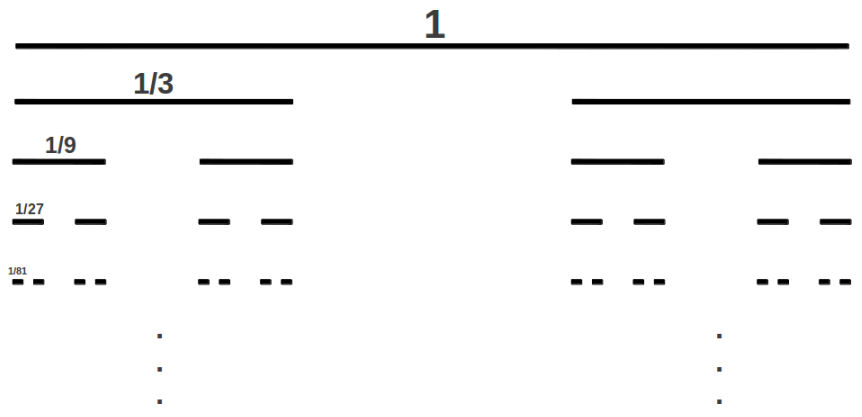
\includegraphics[scale=1]{cantor.jpeg}
\linebreak

Fig 1: Construction of the middle third Cantor Set

\end{center}
Let $E_0$ be the interval [0,1]. Let $E_1$ be the set obtained by deleting the middle third of $E_0$. So that $E_1$ consists of the two intervals [0,1/3] and [2/3,1]. deleting the middle third of these intervals gives $E_2$; thus $E_2$ comprises the four intervals [0,1/9], [2/9,1/3], [2/3,7/9], 8/9,1]. We continue in this way with $E_k$ obtained by deleting the middle third of each interval in $E_{k-1}$.\\
Thus $E_k$ consists of $2^k$ intervals each of length $3^-k$. The middle third Cantor set F consists of the numbers that are in $E_k$ for all k.

Mathematically we write,
\begin{large}
$$F=\cap_{k=0}^{\infty} E_k$$
\end{large}
The Cantor set F may be thought of as the limit of the sequence of the set $E_k$  as k tends to infinity. It is obviously impossible to draw the set F itself with its infinitesimal detail, so 'picture of F' tends to be the picture of some of the $E_k$, which are a good approximation of F when k is reasonably large.\\
At first glance it might appear that we have removed so much of the interval [0,1] during the construction of F, that nothing remains. In fact, F is an uncountably infinite set, which contains infinitely many numbers in every neighbourhood of each of its points. The middle third Cantor set F has following features which are found in many fractals.\\

\begin{enumerate}
\item  \textbf{F is self-similar:}\\
The part of F in the interval [0,1/3] and the past of F in [2/3,1] are both geometrically similar to F scaled by a factor of 1/3. Again the parts of F in each of the four intervals of $E_2$ are similar to F but scaled by a factor 1/9, and so on. The Cantor set contains copies of itself at many different scales.
\item \textbf{F has a 'fine structure':}\\
That is, it contains details at arbitrary small scales. The more we enlarge the picture the more gaps become apparent to the eye.

\item \textbf{F is obtained by a recursive procedure:}\\
Our construction consisted of repeatedly removing the middle third of the intervals. The successive steps give increasingly good approximations '$E_k$' to the set F.

\item \textbf{The geometry of F is not easily described in classical terms:}\\
It is not the locus of the points that satisfy some simple geometric condition, nor is it the set of solutions of any simple equation. It is awkward to describe the local geometry of F. Near each of its points are a large number of other points, separated by the gaps of varying lengths.

\item \textbf{Size of set F:}\\
Although F is in some ways quite a large set (uncountably infinite), its size is not quantized by the usual measures such as length. By any reasonable definition, F has length zero.
\begin{center}

\begin{tabular}{ccl}

$E_0$&$\rightarrow$ & 1 interval length 1   \\
$E_1$&$\rightarrow$ & 2 interval length 1/3 \\
$E_2$&$\rightarrow$ & 4 interval length 1/9 \\
.&. &.\\
.&. &.\\
.&. &.\\
$E_k$ &$\rightarrow$ & $2^k$ interval   length $(1/3)^k$\\


\end{tabular}

\end{center}

$\quad$ Length  of F:
\begin{align*}
l(F)&= 1-2^{0}\left(\frac{1}{3}\right)-2^1\left(\frac{1}{3^2}\right)-2^{2}\left(\frac{1}{3^3}\right)-2^3\left(\frac{1}{3^4}\right)- . . . . .\\
    &= 1-\frac{1}{3}-\frac{1}{3} \left( \frac{2}{3}+ \frac{2^2}{3^2} + \frac{2^3}{3^3}+ . . . . . \right)\\
    &= \frac{2}{3}-\left(\frac{2/3}{1-2/3}\right)\\
	&= \frac{2}{3}- \frac{2}{3}    \\    
    &=0 \\
\end{align*}


\subsection{Example: Von Koch Curve}
\begin{center}

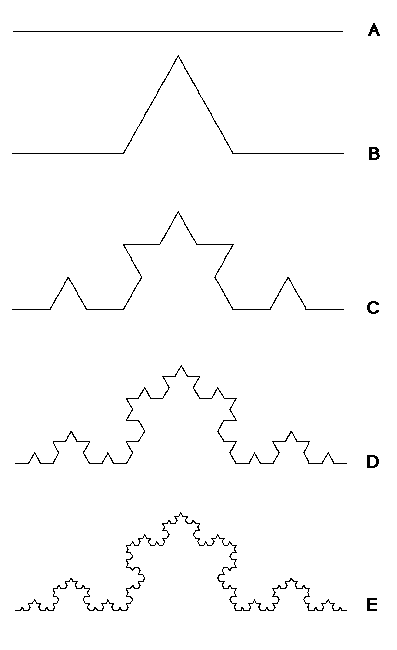
\includegraphics[scale=0.55]{von.png}
\linebreak

Fig 2: Construction of the Koch curve

\end{center}
Let $E_0$ be the line segment of unit length. The set $E_1$ consists of the four segments obtained by removing the middle third of $E_0$ and replacing it by the other 2 sides of the equilateral triangle based on the removed segment. We construct $E_2$ by applying the same procedure to each of the segments in $E_1$ and so on. Thus $E_k$ comes from replacing the middle third of each straight line segment of $E_{k-1}$ by the other two sides of an equilateral triangle. When k is large, the curves $E_{k-1}$ and $E_k$ differ only in fine detail and as k tends to infinity, the sequence of polygonal curves $E_k$ approaches a limiting curve F, called the Von Koch curve. \\



The Von Koch curve F has features in many ways similar to those listed for the middle third Cantor set. Whilst is reasonable to call F a curve, it is much too irregular to have tangents in the classical sense.\\

\begin{center}
\begin{tabular}{cl}
$E_0$ interval & $\rightarrow$ 1  \\
$E_1$ interval & $\rightarrow$ 4/3   \\
$E_2$ interval & $\rightarrow (4/3)^2$    \\
.&.\\
.&.\\
.&.\\
$E_k $ interval & $ \rightarrow (4/3)^k$\\
\end{tabular}

As $k\rightarrow\infty$, length of l(F) $\rightarrow\infty$
\end{center}

So, 'F' has infinite length. On the other hand, 'F' occupies zero area in the plane, so neither length nor area provides a very useful description of the size of 'F'.

\pagebreak
\section{Mathematical background}
We recall the same basic notions from set theory and point set topology here. We generally work in n-dimensional Euclidean space $\mathbb{R}^n$.\\
Let coordinates of points in $\mathbb{R}^n$ be\\
$$x \rightarrow x\ (x_1,x_2,x_3,...,x_n),\quad y \rightarrow y(y_1,y_2,y_3,...,y_n)$$\\

Addition:- $$ x+y=(x_1+y_1,x_2+y_2...,x_n+y_n)$$
Scalar multiplication:- $$\lambda x=(\lambda x_1,\lambda x_2,...,\lambda x_n)$$\\
We use the usual Euclidean distance or metric on $\mathbb{R}^n$\\
$$|x-y|=\left(\sum_{i=1}^{n}|x_i-y_i|\right)^{1/2}$$
closed ball of the centre x and radius r:-\\
$$B(x,r)=\{y:|y-x|<r\}$$\\
If $a<b$:-\\

\begin{tabular}{ll}
Open interval:&$(a,b) \rightarrow{x:a<x<b}$\\
Closed interval:&$[a,b] \rightarrow{x:a\leq x\leq b}$\\
Half-open interval:&$[a,b) \rightarrow{x:a\leq x<b}$\\
\end{tabular}

\subsection{$\delta$ - neighbourhood of set A: $A_\delta$ :}

Set of points within distance $\delta$ of A.\\
$$A_\delta = \{x:|x-y|\leq\delta\}$$ for some y in A.
\subsection{Difference:}  
A set of points in A but not in B is called the 'difference'. Denoted by A\textbackslash B 
\subsection{Complement:}
A set of points not in set A is called complement of set A.\\ 
$ A'=\mathbb{R}^n$ \textbackslash A

\subsection{Supremum: sup A:}
It is the least number 'm' such that $x\leq m$ for every x in A or $\infty$ if no such number exists.

\subsection{Infimum: inf A:}

It is the greatest number 'm' such that $m\leq x$ for all x in A or if not then the infimum of A is infinite.

\subsection{Diameter: $|$A$|$:}

Diameter of a non-empty set is the distance apart from pairs of points in A.

$$|A|= sup\{|x-y|: x,y \in A\}$$

A set is bounded if its diameter is finite.

\subsection{Open set:}

A set is open if, for all points x in A there is some ball B(x,r) centred at x and of positive radius 'r' that is contained in A . e.g. (0,1)

\subsection{Closed set:}

A set is closed if the limit of any convergent sequence of points from the set lies in the set. e.g. [0,1].

\subsection{Boundary: $\partial$A :}
$$\partial A = \bar{A} \backslash int(A)$$

Where $\bar{A}$ = Closure of A $\rightarrow$ Intersection of all closed sets containing a set A.\\
and int(A) = Interior of A $\rightarrow$ Union of all open sets contained in A.\\
The set $\emptyset$ and $\mathbb{R}^n$ are regarded as both open and closed.

\subsection{Compact set:}
A set A is compact if any collection of open sets which covers A (i.e. with union containing A) has a finite sub collection which also covers A.

\subsection{Connected:}

A set is connected if there does not exist an open set U and V such that $U \cup V$ contains A and $A \cap U$ and $A \cap V$ disjoint and non-negative and empty. The set A consists of just one 'piece'. 

\subsection{Totally disconnected:}

A set A is totally disconnected if the connected components of each point consists of just that point.\\

We define the usual mapping function or transformation between sets.\\
Linear transformation:- T: $\mathbb{R}^n \rightarrow \mathbb{R}^n$\\
T(x+y)= T(x)+T(y)\\
$T(\lambda x)= \lambda T(x)$\\
for all $x,y \in \mathbb{R}^n$ and $\lambda \in \mathbb{R}$\\

If S:$\mathbb{R}^n \rightarrow \mathbb{R}^n$ is of the form $S(x)=T(x)+a$ where 'T' is a non-singular linear transformation and 'a' is a point in $\mathbb{R}^n$, then S is called an affine transformation or an affinity. It is a shearing function. If T is a scalar multiple of an orthonormal transformation then T is similarity.
\pagebreak

\section{Measures:}

A measure is just a way of ascribing a numerical size to sets, such that the set can be decomposed into a finite or countable number of pieces in a reasonable way then the size of the whole is the sum of the sizes of the pieces.\\

We call $\mu$ a measure on $\mathbb{R}^n$ if $\mu$  assigns a non-negative number, possibly infinity, to each subset of $\mathbb{R}^n$ such that:\\

\begin{enumerate}
\item $\mu(\phi)=0$
\item $\mu(A) \leq \mu(B) \quad \quad if A \subset B$
\item If $A_1, A_2$ ... is a countable (or finite) sequence of sets then\\

$$\mu \left( \bigcup_{i=1}^{\infty} A_i \right) \leq \sum_{i=1}^{\infty} \mu(A_i)$$
\end{enumerate}
Equality exists if all $A_i$ are disjoint.\\
\end{enumerate}

We call $\mu(A)$ the measure of the set A and think of it as the size of A measured in some way.\\
$$\mu(A\backslash B)= \mu(A)-\mu(B)$$

We think of the support of a measure as the set on which the measure is concentrated. Formally, the support of $\mu$ written 'spt $\mu$' is the smallest closed set X such that $\mu(\mathbb{R}^n\backslash X)=0$.
A measure on a bounded subset of $\mathbb{R}^n$ for which $0< \mu(\mathbb{R}^n)<\infty$ will be called a mass distribution, we think of $\mu(A)$ as the mass of the set A.\\
e.g. Let 'a' be a point in $\mathbb{R}^n$ and define $\mu(A)$ to be 1 if A contains 'a', and '0' otherwise. Then $\mu$ is a mass distribution thought of as a point mass concentrated at 'a'.

\subsection{Lebesgue measure on $\mathbb{R}$:}

Lebesgue measure $L^1$ extends the idea of 'length' to a large collection of subsets of $\mathbb{R}$.\\
For open and closed intervals:
$$L^1(a,b)=L^1[a,b]=b-a$$
Definition:-\\
$$L^1(A)=inf\left\lbrace \sum_{i=1}^{\infty}(b_i-a_i): A \subset \bigcup_{i=1}^{\infty} [a_i,b_i] \right\rbrace$$
We look at all coverings of A by countable collections of intervals and take the smallest total interval length possible. It is defined for a large class of sets called 'the Lebesgue measurable sets' but not for all subsets of $\mathbb{R}$.\\
Lebesgue measure on $\mathbb{R}^n$:-
The n-dimensional Lebesgue measure $L^n$ may be thought of as the extension of n-dimensional volume to a large class of sets.\\

$$L^n(A)=inf\left\lbrace \sum_{i=1}^{\infty} Vol^n(A_i): A \subset \bigcup_{i=1}^{\infty} A_i \right\rbrace$$
Where,

$$Vol^n(A_i)=(b_1-a_1)(b_2-a_2)....(b_n-a_n)$$
for $A=\lbrace (x_1,x_2....x_n) \in \mathbb{R}^n : a_i \leq x_i \leq b_i \rbrace$

$$Area(A)\equiv L^2(A)$$
$$Vol(A)\equiv L^3(A)$$

\subsection{Hausdorff measure:}

If $\lbrace U_i \rbrace$ is accountable (or finite) collection of sets of diameter at most $\delta$ that cover 'F', i.e. F $\subset \cup_{i=1}^{\infty} U_i$ with $0 \leq |U_i| \leq \delta$ for each 'i', we say that $\lbrace U_i \rbrace$ is a $\delta$-cover of 'F'.\\

Suppose that 'F' is a subset of $\mathbb{R}^n$ and 'S' is a non-negative number . Then for any $\delta > 0$, then we define\\

$$H_{\delta}^s(F)=inf \left\lbrace \sum_{i=1}^{\infty} |U_i|^s : \lbrace U_i \rbrace \, is \, a \, \delta \, cover \, of \, F \, \right\rbrace $$


Thus we look at all covers of F by sets of diameter at most $\delta$ and seek to minimize the sum of the $s^{th}$ power of the diameters. As $\delta$ decreases, the class of permissible covers of F is reduced. Therefore the infimum $H_{\delta}^s(F)$ increases and so approaches a limit as $\delta \rightarrow 0$, we write

$$H^s(F)= \lim_{\delta \rightarrow 0} H_{\delta}^s(F) $$

This limit exists for any subset 'F' of $\mathbb{R}^n$, though the limiting value can be 0 or $\infty$. We call $H^s(F)$ the s-dimensional Hausdorff measure of F.

\subsection{Hausdroff dimension:}

How does the Hausdorff measure $H^s(F)$ behave as a function of '$\delta$' for a given set F? From the definition of $H_{\delta}^s(F)$ , for F $\subset$ $\mathbb{R}^n$ and $\delta < 1$, $H_{\delta}^s(F)$ is non-increasing with 's', so $H^s(F)$ is also non-increasing.\\

Is $t<s$ and $\lbrace U_i \rbrace$ is a $\delta$-cover of F we have 

$$\sum_i |U_i|^t = \sum_i |U_i|^{t-s} |U_i|^s \leq \delta^{t-s} \sum_i |U_i|^s $$ 

Taking infima:- 

$$H_{\delta}^s(F) \leq \delta^{t-s} H_{\delta}^s(F)$$

letting $\delta \rightarrow 0$ :-   \quad if $H^s(F) < \infty$ then $H^t(F)=0$

Thus a graph of $H^s(F)< \infty$ vs s shows a critical value of s at which $H^s(F)$ jumps from $\infty$ to 0. This value of s is called the Hausdorff dimension of F ($dim_H F$).\\

$$ dim_H F =inf \left\lbrace s \geq 0; H^s(F)=0 \right\rbrace = sup \left\lbrace s: H^s(F)=\infty \right\rbrace$$ 

At $ s=dim_H F, 0\leq H^s(F) \leq \infty$

\begin{center}

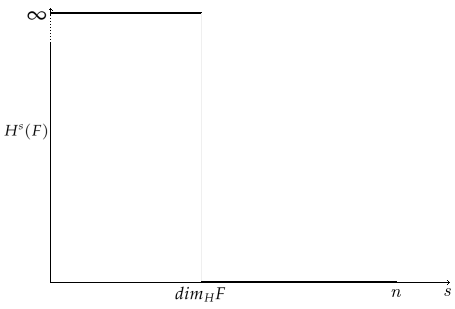
\includegraphics[scale=1]{1111.png}
\linebreak

Fig 3: Hausdorff dimension

\end{center}

\newpage


\section{Path Integrals in Quantum mechanics}

A fundamental question in quantum mechanics is how does the state of a particle evolve with time? That is, the determination of the   $|\psi(t)\rangle$ given some initial state $|\psi(t_0)\rangle$. Schrödinger’s equation is one way of finding it. A well-established method of solution, after the entire eigen spectrum of $\hat{H}$ is known, is to decompose the initial state into this eigenbasis, apply time evolution to each and then reassemble the eigenstates.

$$|\psi(t)\rangle = \sum_{n=0}^{\infty} e^{-iE_n t/\hbar} \langle n|\psi(t_0) \rangle |n \rangle$$

This Hamiltonian formalism works in many cases. In classical mechanics, however , the Lagrangian formalism is known to be equivalent to the Hamiltonian one.\\

Let a given trajectory x(t) be associated with a transition probability amplitude of course, by quantum mechanics, we cannot speak of the particle taking any well-defined trajectory between two points $(x_0,t_0)$ and $(x',t')$. Instead we can only speak of the probability of finding the particle at these locations, which is related to wave function $|\psi(x_0,t_0)\rangle$ and $|\psi(x',t')\rangle$. Feynman's insight was this- the total transition probability amplitude can be obtained by summing the amplitudes of the particle having taken any individual path. If the quantity $\langle \psi(x_0,t_0)|\psi(x_0,t_0)\rangle$ can be calculated in the method suggested by Feynman, the time-evolution of the state can be determined by considering contributions from all possible states and the problem is solved. Below, the kets are eigenstates of the position operator, such that integration over all x spans the entire basis.

$$|\psi (x,t') \rangle = \int_{-\infty}^{\infty} \langle \psi(x_0,t_0)|\psi(x_0,t_0)\rangle |\psi(x',t')\rangle dx'  $$


Known as the path integral formulation of quantum mechanics, this method gives the same results as those dictated by the Schrödinger picture, but also illuminates some of the deeper aspects of quantum mechanics . We define the propagator of a quantum system between two spacetime points $(x',t')$ and $(x_0,t_0)$ to the probability transition amplitude between the wavefunction evaluated at those points.

$$U(x',t';x_0,t_0) = \rangle \psi (x',t')| \psi (x_0,t_0)$$

If the Hamiltonian carries no explicit time-dependence, we can relabel the first value $t_0=0$ and work only with elapsed time $t=t'-t_0$. The propagator above along with an initial state ket fully describe the evolution of a system over time. The path integral method, as we are about to see, is an explicit way to construct this propagator.\\
We consider possible trajectories x(t) of a particle moving through a time-independent potential V(x) with end points fixed at $(x',t')$ and $(x_0,t_0)$ (in any number of dimensions). An infinite continuum of such trajectories are possible, each with classical action S[x(t)]. Feynman posits that the contribution to the propagator from a particular trajectory is $exp(iS[x(t)]/\hbar)$. That is, every possible path contributes with equal amplitude to the propagator, but with a phase related to the classical action. Summing over all possible trajectories, we arrive at the propagator. The normalization constant A(t) is independent of any individual path and therefore depends only on time.

$$U(x',t';x_0,t_0) = A(t) \sum_{all \, trajectories} e^{iS[x(t)]/\hbar}$$

\newpage

\section{Dimension of a quantum-mechanical path}
 \textbf{L. Abbott and M. Wise}
 
 \subsection{Introduction:}
 
 In quantum mechanics, the distance which a particle travels in a fixed period of time depends on the resolution of the detecting apparatus which is used to track the particle. Similar correlations between distance and resolution are found in curves which are given by everywhere continuous but nowhere differentiable functions, like the Koch curve we saw as an example of fractal. The similarity between this curve and the quantum mechanical particle become apparent when we consider viewing the Koch curve with finite spatial resolution. In this case, the infinitely many wiggles in the curve which are smaller than some minimum length $\Delta x$, cannot be detected and the measured length of the curve resolves distances greater than some scale $\Delta x$ and measure its length to be l. Then if we improve our resolution so that $\Delta x'=(1/3) \Delta x$, the next level of wiggles in the curve will become visible and we will measure a new length $l'=(4/3)l$.\\
 Since the conventional definition of length, when applied to curves like the Koch curve, gives a quantity which depends on the resolution with which the curve is examined(even for very small 
$ \Delta x$), it is not very useful. Hausdorff proposed a modified definition of length to be used in these cases.\\

The Hausdorff length L is given by 
$$L=l(\Delta x)^{D-1}$$

Where, \\
D:\hspace{7mm}  A number chosen so that L will be independent of $\Delta x$\\
 l:\hspace{10mm} Usual length measured for $\Delta x$ resolution.\\
$\Delta x$:\hspace{5mm} Resolution of length measurement.\\

Hausdorff length reduces to the usual concept of length when D=1. For the Koch curve, we determined D by requiring that,

$$L'=l'(\Delta x')^{D-1}= \frac{4}{3}l \left( \frac{1}{3} \Delta x \right)^{D-1} = l(\Delta x)^{D-1}$$

$$\frac{4}{3} \left( \frac{1}{3} \right)^{D-1} =1$$

$$D= \frac{ln4}{ln3}$$

Clearly the Hausdorff definition of length is more practical than the conventional one because it eliminates the resolution or scale dependence of the measured value of the length of a curve.\\
To define the quantum mechanical path of a particle we imagine measuring the position of a free particle with a spatial resolution $\Delta x$ at times separated by an interval $\Delta t$. The path is then defined as the curve determined by drawing straight lines between the points where the particle was located at sequential times. To be more precise one should draw straight lines between the centres of regions within which the particle is known to lie, since we are working with an uncertainty $\Delta x$. At the classical level, this path will just be a straight line with dimension D=1 (or in the case of a particle at rest, a point of zero dimension).\\

At the quantum level, the localization of a particle within a region of size $\Delta x$ results, according to the Heisenberg uncertainty principle, in an uncertainty in the momentum of order $\hbar/\Delta x$.  Thus as the particle is more and more precisely located in space, its path will become increasingly erratic. Of course, in quantum mechanics, we can only speak of a particle's path in the statistical sense and we must work with average values. If we measure the position of a particle at time $t_1=t_0+\Delta t$, $t_0+2\Delta t$, ...,$t_N= t_0+N\Delta t$ with $T=t_N-t_0$.\\

$\therefore T=N\Delta t$, the length of the particle's path will be\\

$$\langle l \rangle = N \langle \Delta l \rangle$$

where $\langle \Delta l \rangle$ is the average distance which the particle travels in time $\Delta t$.

\subsection{CASE I: Zero average momentum:-}

(In the classical limit, the particle is at rest).\\
In the sec. II of paper, it has been proved for particle with zero average momentum that:-
$$\langle \Delta l \rangle \propto \frac{\hbar \Delta t}{m \Delta x}$$
$$\langle  l \rangle \propto \frac{\hbar T}{m \Delta x}$$

Following Hausdorff, we can introduce a modified definition of length,\\

$$\langle  L \rangle= \langle l \rangle (\Delta x)^{d-1}$$

$$\langle  L \rangle \propto \frac{\hbar T}{m \Delta x}  \rangle (\Delta x)^{d-1}$$

$$\langle  L \rangle \propto (\Delta x)^{D-2}$$

Requiring that $\langle L \rangle$ be independent of $\Delta x$ gives, Hausdorff dimension of particle to be, D=2. The path of a quantum mechanical particle is therefore a fractal of dimension 2.

\subsection{CASE II: Non-zero average momentum:-}

The Koch curve has another interesting property, which under certain circumstances, is shared by the quantum mechanical particle path. This is self similarity. The path of the particle will be self-similar if

$$\langle \Delta l \rangle \propto \Delta x$$

also from previous case $\langle \Delta l \rangle \propto \frac{\hbar \Delta t}{m \Delta x}$

$$\therefore \Delta t \propto \frac{m (\Delta x)^2}{\hbar}$$

This is required for the resulting path to be self-similar. Refer section II of paper for justification for $\Delta l \propto \Delta x$, and section III for usage of $\Delta t \propto m (\Delta x)^2 / \hbar$ for the case of non-zero average momentum.\\
Thus, just as fractal nature of the quantum mechanical path reflects the Heisenberg uncertainty principle, the condition for self-similarity, above proportionality is a reflection of the underlying dynamics $E=p^2 /2m$.\\

From section III of the paper, the last equation gives the Hausdorff length of a particle with $\mathbf{p_{av}}$ as average momentum.

$$ \langle L \rangle = N \langle \Delta l \rangle (\Delta x)^{D-1}$$

After substituting the value of $\langle \Delta l \rangle$, we get;

$$\langle L \rangle = \frac{|\mathbf{p_{av}}|T}{m} \int_{R^3} d^3 y \left| \frac{\mathbf{p_{av}}}{|\mathbf{p_{av}}|} + \frac{\hbar \mathbf{y}}{2|\mathbf{p_{av}}|} (\Delta x)b     \right| |F(\mathbf{y},b)|^2 (\Delta x)^{D-1}  $$

where 'y' is a dimensionless position variable.

$$b= \frac{\hbar \Delta t}{2m (\Delta x)^2}$$

$F(\mathbf{y},b)$ is the wavefunction in new variables.

Requiring that the Haudorff length $\langle L \rangle$ be independent of $\Delta x$ gives\\

 D=1 when $\Delta x>> \frac{\hbar}{|\mathbf{p_{av}}|}$ and\\

 D=2 when $\Delta x<< \frac{\hbar}{|\mathbf{p_{av}}|}$\\

These are respectively the classical and quantum mechanical limits. IN the region between these limits the Hausdorff dimension D is not well defined since it is rapidly varying with $\Delta x$.

\newpage

\section{Charged Particle in a magnetic field}

The 3 dimensional propagator for a particle moving from \textbf{y} to \textbf{x} is given by

$$G(\textbf{x},t;\textbf{y}) = \int_{\textbf{y},0}^{\textbf{x},t} d\textbf{x}(\tau) e^{iS[\textbf{x}(\tau)/\hbar]}$$

Where $S[\textbf{x}(\tau)$ is the action for an arbitrary path $\textbf{x}(\tau)$.\\

In the absence of magnetic fields we already know that $S$ has the form.

$$S[\textbf{x}(\tau) = \int_0^t L \left( \textbf{x}, \frac{d\textbf{x}}{dt} \right) d\tau$$

where,

$$L = \frac{1}{2} m \left( \frac{d\textbf{x}}{dt} \right)^2 - V(\textbf{x}) $$


In presence of a magnetic field $\textbf{B}$, derivable from vector potential $\textbf{A}$, the only change in L is

$$L = \frac{1}{2} m \left( \frac{d\textbf{x}}{dt} \right)^2 - \frac{e}{c} 
\frac{d\textbf{x}}{dt} \cdot \textbf{A}  - V(\textbf{x})$$

In the action, there will appear an additional term
 $$\frac{e}{c} \int_0^t d\tau \frac{d\textbf{x}}{dt} \cdot  \textbf{A}  = \frac{e}{c} \int_0^t d\textbf{x} \cdot \textbf{A}$$

The way to check whether the proposed propagator with the Lagrangian given above is correct is to look at the expression for G as the limit:


\begin{eqnarray}
G(\textbf{x},t;\textbf{y}) = \lim_{N\rightarrow \infty} \int d^3x_1....d^3x_N \left( \frac{m}{2 \pi i \hbar \epsilon} \right)^{3(N+1)/2} \nonumber \\
\times exp \left\lbrace \frac{i\epsilon}{\hbar} \sum_{j=0}^N \left[ \frac{m}{2} \left( \frac{\textbf{x}_{j+1}-\textbf{x}_j}{\epsilon} \right)^2 -V(\textbf{x}_j) \right] + vector\; potential\; term\; \right\rbrace \nonumber
\end{eqnarray}


(Refer th book by Schulman, chapter 1 for origin of this equation)

where,$$\epsilon = \frac{t}{N+1}$$

Now, the extra term in S is

$$\frac{ie}{\hbar c} \int d\textbf{x} \cdot \textbf{A} = \frac{ie}{\hbar c} \sum_{j=0}^N (\textbf{x}_{j+1} - \textbf{x}_j) \cdot \textbf{A}(\textbf{x})$$


But it is not clear whether $\textbf{A}(\textbf{x})$ should be evaluated at $\textbf{x}_j$, $\textbf{x}_{j+1}$ or somewhere in between. It turns out that only when $\textbf{A}(\textbf{x})= \frac{1}{2} [\textbf{A}(\textbf{x}_j) + \textbf{A}(\textbf{x}_{j+1})]$ or $ \textbf{A}(\textbf{x})$ evaluated at midpoint i.e. $\frac{1}{2} (\textbf{x}_j + \textbf{x}_{j+1})$ works to give the correct Schrödinger equation from the above propagator. We now show that how it works for the midpoint value of $\textbf{A}$.\\

The way we check the validity of this method for handling magnetic fields is the same way Feynman first verified the entire formalism. Namely, take a wave-function at time T, $\psi (\textbf{y},T)$, propagate it to time $T+\epsilon$ by means of a putative path integral propagator, and see if this evolution is the same as that given by the Schrödinger equation. For this purpose we take as propagator the quantity under the limit operation for $G(\textbf{x},t,\textbf{y})$ given above for the case N=0 (i.e. for a single infinitesimal time stop) and include the vector potential $\textbf{A}[\frac{1}{2} (\textbf{x}_j + \textbf{x}_{j+1})]$ contribution. This will be used to propagate $\psi$ for a time $\epsilon$ and we shall eventually let $\epsilon$ go to zero to allow comparison with the time derivative operator of Schrödinger’s equation. If the theory is correct we should therefore have

$$\psi(\textbf{x},T+\epsilon) = G(\textbf{x},t:\textbf{y}) \psi(\textbf{y},T)$$


\begin{multline}
 \psi(\textbf{x},T+\epsilon) =  \int d^3 y \left( \frac{m}{2 \pi i \hbar \epsilon} \right)^{3/2} \nonumber \\ \times exp \left\lbrace \frac{i\epsilon}{\hbar} \left[ \frac{m}{2} \left( \frac{\textbf{x}-\textbf{y}}{\epsilon} \right)^2 -V(\textbf{y}) \right] + \frac{ie}{\hbar c} (\textbf{x}-\textbf{y}) \cdot \textbf{A} \left( \frac{1}{2} \textbf{x} + \frac{1}{2} \textbf{y} \right)  \right\rbrace \psi(\textbf{y},T) \nonumber 
\end{multline}


Now, we change he variable and expand $\psi(\textbf{y},T)$, $\textbf{A}$ and V about origin.
$$\textbf{$\xi$} = \textbf{y} - \textbf{x}  $$
$$\therefore d^3y=d^3 \xi$$









\begin{multline}
\psi(\textbf{x},T+\epsilon) =\left( \frac{m}{2 \pi i \hbar \epsilon} \right) \int d^3 \xi exp{\left[ \frac{im \xi^2}{2 \epsilon \hbar} \right]} \times  exp \left\lbrace \frac{-i \epsilon}{\hbar} V(\textbf{x}) - \frac{i \epsilon}{\hbar} \nabla V(\textbf{x}) \cdot  \boldsymbol{\xi}  + \dots \right\rbrace \\ 
\times exp \left\lbrace \frac{-i \epsilon}{\hbar} \left[ \boldsymbol{\xi} \cdot \textbf{A}(\textbf{x}) + \frac{1}{2} (\boldsymbol{\xi} \cdot \nabla) \textbf{A}(\textbf{x})+ \dots \right]  \right\rbrace \nonumber \\ \times  \left\lbrace \psi(\textbf{x},T) + \boldsymbol{\xi} \cdot \nabla \psi + \frac{1}{2} \sum_{m,n=1}^3 \xi_m \xi_n \frac{\partial^2 \psi}{\partial x_m \partial x_n} + \dots \right\rbrace
\end{multline}












We are considering the integral in the limit $\epsilon \rightarrow 0$. We are hence only interested in terms of first order in $\epsilon$.\\

The factor $\xi$ which appear inside the integral have an effective size in terms of $\epsilon$ as these terms together with $exp[\frac{im \xi^2}{2 \epsilon \hbar}]$ makes up the form $\int e^{-x^2} x^n dx$.[2]\\


In turns out that $\xi$ is of the order $\sqrt{\epsilon}$.\\

After solving these integrals and neglecting higher order of '$\epsilon$' terms, we get is the following

\begin{multline}
\psi(\textbf{x},T+\epsilon) = \psi - \frac{i \epsilon}{\hbar} V \psi + \frac{\epsilon e}{2mc} \psi  \nabla \cdot \textbf{A} - \frac{i \epsilon e^2}{2 \hbar mc^2} \textbf{A}^2 \psi + \frac{i \epsilon \hbar}{2m} \nabla^2 \psi + \frac{\epsilon e}{mc} (\textbf{A} \cdot \nabla) \psi \nonumber
\end{multline}


Take $\psi \equiv \psi(\textbf{x},T)$ to L.H.S. and multiply whole equation by $i\hbar/c$\\

$$\lim_{\epsilon \rightarrow 0} \frac{\psi(\textbf{x},T+\epsilon)-\psi(\textbf{x},T)}{\epsilon} =\frac{\partial \psi}{\partial t} $$

\begin{multline}
i\hbar \frac{\partial \psi}{\partial t} = -\frac{\hbar^2}{2m} \nabla^2 \psi + \frac{\epsilon e}{mc} (\textbf{A} \cdot \nabla) \psi + \frac{i \hbar e}{2mc} \psi ( \nabla \cdot \textbf{A}) + \frac{e^2}{2mc^2} \textbf{A}^2 \psi + V \psi \nonumber
\end{multline}

Which is same as:- \\

$$i \hbar \frac{\partial \psi}{\partial t} =\frac{1}{2m} \left( \textbf{p}- \frac{e}{c} \textbf{A} \right)^2  \psi + V \psi $$

with $\textbf{p}= -i \hbar \nabla$\\

$\therefore$ We have recovered the Schrödinger’s equation from the path integral method.

\newpage

\section{Problem Statement:}

We have seen that the path integral method for a particle in magnetic field gives the correct Schrödinger’s equation only when


i)The vector potential $\textbf{A}$ was evaluated at the midpoint of initial and final point.

ii)The vector potential evaluated at the average of the initial and final point values.

If, lets say we try doing it for initial point i.e. extra term in action, S as

$$\int \textbf{A} \cdot d\textbf{x} = \sum_{j=0}^N (\textbf{x}_{j+1} -\textbf{x}_j) \cdot \textbf{A}(\textbf{x}_j)$$

it leads to the Schrödinger equation

$$i \hbar \frac{\partial \psi}{\partial t} =\frac{1}{2m} \left( \textbf{p}- \frac{e}{c} \textbf{A} \right)^2  \psi + V \psi + \frac{i \hbar e}{2mc} \psi \nabla \cdot \textbf{A} $$

which is  incorrect.\\

This is absurd because for example in Riemann integral to find area under a curve, when we split the 'x' axis into intervals, it doesn't matter we take ($x_2-x_1$)f($x_1$) or ($x_2-x_1$)f($x_2$) where $x_1$ and $x_2$ are initial and final points on an interval.

$$\sum_{j=0}^N (x_{j+1}-x_j)f(x_j^{\ast})$$


The value of above summation converges to the same number called $\int_a^b f(x)dx$ as long as $(x_{j+1}-x_j) \rightarrow 0$ and $x_j \leq x_j^{\ast} \leq x_{j+1} $

So, our integral of vector potential $\int \textbf{A} \cdot d\textbf{x}$ is surely not a Riemann integral.\\

In the study of Brownian motion, K. Ito found similar problem in attempting to define an integral

$$\int_a^b f[x(t)] dx$$

Where $x(t)$ is a Brownian motion path. He chose to define this integral as

$$\lim_{n \rightarrow \infty} \sum_{j=0}^{n-1} (x_{j+1}-x_j) f(x_j)$$

$$x_j= x \left( a+j \frac{(b-a)}{n} \right) , \quad x_n=x(b), \quad x(0)=x(a)=x_a$$

He then found that

$$\int_{x_a}^{x_b} \frac{d\phi}{dx} dx =\phi(x_b) - \phi (x_a) - \frac{1}{2} \int_a^b \frac{d^2\phi[x(t)]}{dx^2} dt$$

But for the specific case of midpoint, the anomalous third term vanishes and it reduces to familiar form. So even Ito integral (above) cannot be an option to evaluate our vector potential $\int \textbf{A} \cdot d\textbf{x} $.\\

So, the problem is to find a general way to evaluate this integral without using the specific cases of midpoint or average of $\textbf{A}$. So, considering the fact that quantum mechanical paths are fractal, we want to formulate a method using fractal geometry and calculus of fractal curves to deal with this kind of integrals.


\newpage

\section*{References:}

\begin{enumerate}


\item K. Falconer, Fractal Geometry: Mathematical Foundation and Application, 2nd Ed. (John Wiley and Sons, 2003)

\item L.S. Schulman, Techniques and Applications of Path Integration (John Wiley and Sons. NY, 1981)

\item L. F. Abbott and M. B. Wise, Dimension of quantum mechanical path, Am. J. Phys. 49(1) (1981) 37-39

\item D. Perepelitsa, Path Integral in Quantum Mechanics.\\ (http://web.mit.edu/dvp.www/Work/8.06/dvp-8.06-paper.pdf)

\item R. Shankar, Principles of Quantum Mechanics, 2nd Ed. (Springer, New Delhi, 2010)




\end{enumerate}



\end{document}